% Generated by tools/gen_figures.py; do not edit by hand.
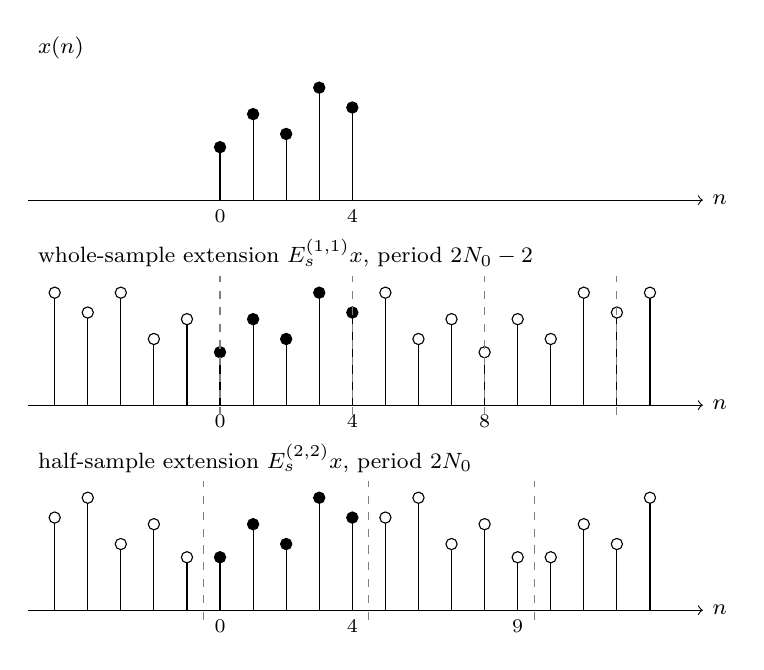
\begin{tikzpicture}[x=0.42cm,y=0.42cm]
  \draw[->] (-5.8,-0.0) -- (14.6,-0.0) node[right,font=\footnotesize] {$n$};
  \node[anchor=west,font=\footnotesize] at (-5.8,4.6) {$x(n)$};
  \draw (0,-0.0) -- (0,1.6);
  \fill[black,draw=black] (0,1.6) circle (0.17);
  \draw (1,-0.0) -- (1,2.6);
  \fill[black,draw=black] (1,2.6) circle (0.17);
  \draw (2,-0.0) -- (2,2.0);
  \fill[black,draw=black] (2,2.0) circle (0.17);
  \draw (3,-0.0) -- (3,3.4);
  \fill[black,draw=black] (3,3.4) circle (0.17);
  \draw (4,-0.0) -- (4,2.8);
  \fill[black,draw=black] (4,2.8) circle (0.17);
  \node[below,font=\scriptsize] at (0,-0.0) {0};
  \node[below,font=\scriptsize] at (4,-0.0) {4};
  \draw[->] (-5.8,-6.2) -- (14.6,-6.2) node[right,font=\footnotesize] {$n$};
  \node[anchor=west,font=\footnotesize] at (-5.8,-1.6000000000000005) {whole-sample extension $E_s^{(1,1)}x$, period $2N_0-2$};
  \draw (-5,-6.2) -- (-5,-2.8000000000000003);
  \fill[white,draw=black] (-5,-2.8000000000000003) circle (0.17);
  \draw (-4,-6.2) -- (-4,-3.4000000000000004);
  \fill[white,draw=black] (-4,-3.4000000000000004) circle (0.17);
  \draw (-3,-6.2) -- (-3,-2.8000000000000003);
  \fill[white,draw=black] (-3,-2.8000000000000003) circle (0.17);
  \draw (-2,-6.2) -- (-2,-4.2);
  \fill[white,draw=black] (-2,-4.2) circle (0.17);
  \draw (-1,-6.2) -- (-1,-3.6);
  \fill[white,draw=black] (-1,-3.6) circle (0.17);
  \draw (0,-6.2) -- (0,-4.6);
  \fill[black,draw=black] (0,-4.6) circle (0.17);
  \draw (1,-6.2) -- (1,-3.6);
  \fill[black,draw=black] (1,-3.6) circle (0.17);
  \draw (2,-6.2) -- (2,-4.2);
  \fill[black,draw=black] (2,-4.2) circle (0.17);
  \draw (3,-6.2) -- (3,-2.8000000000000003);
  \fill[black,draw=black] (3,-2.8000000000000003) circle (0.17);
  \draw (4,-6.2) -- (4,-3.4000000000000004);
  \fill[black,draw=black] (4,-3.4000000000000004) circle (0.17);
  \draw (5,-6.2) -- (5,-2.8000000000000003);
  \fill[white,draw=black] (5,-2.8000000000000003) circle (0.17);
  \draw (6,-6.2) -- (6,-4.2);
  \fill[white,draw=black] (6,-4.2) circle (0.17);
  \draw (7,-6.2) -- (7,-3.6);
  \fill[white,draw=black] (7,-3.6) circle (0.17);
  \draw (8,-6.2) -- (8,-4.6);
  \fill[white,draw=black] (8,-4.6) circle (0.17);
  \draw (9,-6.2) -- (9,-3.6);
  \fill[white,draw=black] (9,-3.6) circle (0.17);
  \draw (10,-6.2) -- (10,-4.2);
  \fill[white,draw=black] (10,-4.2) circle (0.17);
  \draw (11,-6.2) -- (11,-2.8000000000000003);
  \fill[white,draw=black] (11,-2.8000000000000003) circle (0.17);
  \draw (12,-6.2) -- (12,-3.4000000000000004);
  \fill[white,draw=black] (12,-3.4000000000000004) circle (0.17);
  \draw (13,-6.2) -- (13,-2.8000000000000003);
  \fill[white,draw=black] (13,-2.8000000000000003) circle (0.17);
  \node[below,font=\scriptsize] at (0,-6.2) {0};
  \node[below,font=\scriptsize] at (4,-6.2) {4};
  \node[below,font=\scriptsize] at (8,-6.2) {8};
  \draw[dashed,gray] (0,-6.5) -- (0,-2.3000000000000003);
  \draw[dashed,gray] (4,-6.5) -- (4,-2.3000000000000003);
  \draw[dashed,gray] (8,-6.5) -- (8,-2.3000000000000003);
  \draw[dashed,gray] (12,-6.5) -- (12,-2.3000000000000003);
  \draw[->] (-5.8,-12.4) -- (14.6,-12.4) node[right,font=\footnotesize] {$n$};
  \node[anchor=west,font=\footnotesize] at (-5.8,-7.800000000000001) {half-sample extension $E_s^{(2,2)}x$, period $2N_0$};
  \draw (-5,-12.4) -- (-5,-9.600000000000001);
  \fill[white,draw=black] (-5,-9.600000000000001) circle (0.17);
  \draw (-4,-12.4) -- (-4,-9.0);
  \fill[white,draw=black] (-4,-9.0) circle (0.17);
  \draw (-3,-12.4) -- (-3,-10.4);
  \fill[white,draw=black] (-3,-10.4) circle (0.17);
  \draw (-2,-12.4) -- (-2,-9.8);
  \fill[white,draw=black] (-2,-9.8) circle (0.17);
  \draw (-1,-12.4) -- (-1,-10.8);
  \fill[white,draw=black] (-1,-10.8) circle (0.17);
  \draw (0,-12.4) -- (0,-10.8);
  \fill[black,draw=black] (0,-10.8) circle (0.17);
  \draw (1,-12.4) -- (1,-9.8);
  \fill[black,draw=black] (1,-9.8) circle (0.17);
  \draw (2,-12.4) -- (2,-10.4);
  \fill[black,draw=black] (2,-10.4) circle (0.17);
  \draw (3,-12.4) -- (3,-9.0);
  \fill[black,draw=black] (3,-9.0) circle (0.17);
  \draw (4,-12.4) -- (4,-9.600000000000001);
  \fill[black,draw=black] (4,-9.600000000000001) circle (0.17);
  \draw (5,-12.4) -- (5,-9.600000000000001);
  \fill[white,draw=black] (5,-9.600000000000001) circle (0.17);
  \draw (6,-12.4) -- (6,-9.0);
  \fill[white,draw=black] (6,-9.0) circle (0.17);
  \draw (7,-12.4) -- (7,-10.4);
  \fill[white,draw=black] (7,-10.4) circle (0.17);
  \draw (8,-12.4) -- (8,-9.8);
  \fill[white,draw=black] (8,-9.8) circle (0.17);
  \draw (9,-12.4) -- (9,-10.8);
  \fill[white,draw=black] (9,-10.8) circle (0.17);
  \draw (10,-12.4) -- (10,-10.8);
  \fill[white,draw=black] (10,-10.8) circle (0.17);
  \draw (11,-12.4) -- (11,-9.8);
  \fill[white,draw=black] (11,-9.8) circle (0.17);
  \draw (12,-12.4) -- (12,-10.4);
  \fill[white,draw=black] (12,-10.4) circle (0.17);
  \draw (13,-12.4) -- (13,-9.0);
  \fill[white,draw=black] (13,-9.0) circle (0.17);
  \node[below,font=\scriptsize] at (0,-12.4) {0};
  \node[below,font=\scriptsize] at (4,-12.4) {4};
  \node[below,font=\scriptsize] at (9,-12.4) {9};
  \draw[dashed,gray] (-0.5,-12.700000000000001) -- (-0.5,-8.5);
  \draw[dashed,gray] (4.5,-12.700000000000001) -- (4.5,-8.5);
  \draw[dashed,gray] (9.5,-12.700000000000001) -- (9.5,-8.5);
\end{tikzpicture}
